% Provenance (never printed): see sources/outline_sources.md (Year 3:
% spectral signatures; optical, thermal and radar sensors; radar
% interferometry; digital elevation models; GIS operations).
% Brief: sources/book5/BRIEFS.md, ch. 25. Curves from figdata/bachelor-3/
% spectral_signatures.py (ECOSTRESS spectra and the Landsat 8 OLI bands),
% thermal_ir.py (Planck's law, brightness temperatures, a mixed pixel),
% insar_mogi.py (the wrapped interferogram of a Mogi source) and
% varden_gis.py (slope, aspect and an overlay on the Varden Hills, from
% figdata/shared/region.py, read only). Exercise and problem values in the
% Book 5 scratch calculator calc/ch25.py. Mount Halvren, its lava flows and
% its fumaroles are invented. The brief's overlay (slope > 15 degrees on
% limestone within 200 m of the river) is empty on the Varden model: the
% valley floor is flat; the printed overlay uses the shale within 1 km.
\chapter{Télédétection et SIG}\label{ch:b3:remote-sensing-gis}

En 1997, le sol d'une région sauvage de la chaîne des Cascades, près de
l'ensemble de volcans appelé les Three Sisters, commença à se soulever. En 2001,
son centre se trouvait \qty{15}{cm} plus haut. Aucun volcan ne s'élève directement
au-dessus du soulèvement. La dernière éruption de la zone remontait à 1~500 ans.
Le soulèvement n'a été repéré par personne qui le parcourait~: il apparut sous la forme
d'une cible d'anneaux colorés lorsque des images radar de la région, prises depuis l'orbite
à plusieurs années d'intervalle, étaient combinées. Les anneaux situaient le magma intrusif
entre 6 et \qty{7}{km} de profondeur~; en mars 2004, un essaim de plus de 300 petits séismes
s'est produit à proximité de leur centre. Ce chapitre explique comment un satellite mesure
une variation de quelques centimètres depuis des centaines de kilomètres d'altitude, ce que voient
du sol les autres capteurs en orbite, et comment les cartes qu'ils produisent sont combinées
dans un système d'information géographique.
% ledger: usgs:insar-fs

\begin{recall}
Le spectre électromagnétique, la loi de Planck du corps noir, l'émissivité
et la loi de Kirchhoff, la réflectance et l'interférence des ondes figurent dans les
volumes de physique. La télédétection, les images satellitaires, les projections
cartographiques et le positionnement par satellite figurent dans les manuels scolaires. Les
fenêtres atmosphériques et les bandes photométriques figurent dans le volume de première année,
dans son chapitre sur les télescopes~; le modèle numérique de terrain et le système
d'information géographique qui le stocke figure dans son chapitre sur les cartes géologiques~;
la première carte radar du déplacement d'un séisme, dans son chapitre sur la source sismique.
La source de Mogi d'un réservoir magmatique en gonflement figure dans le volume de deuxième
année, dans son chapitre sur les éruptions volcaniques.
\end{recall}

\section{Signatures spectrales et capteurs optiques}\label{sec:b3:remote-sensing-gis:optical}

La lumière solaire qui atteint le sol est en partie absorbée et en partie réfléchie,
dans des proportions qui dépendent de la longueur d'onde et de la composition du sol.
Un capteur en orbite mesure la lumière réfléchie dans quelques intervalles de
longueurs d'onde, ses bandes, et les rapports entre les bandes identifient la
surface.

\begin{definition}[Signature spectrale]\label{def:b3:remote-sensing-gis:signature}
La \emph{signature spectrale}\index{signature spectrale} d'un matériau est
sa réflectance en fonction de la longueur d'onde, $R(\lambda)$, la fraction du
rayonnement incident qu'elle réfléchit. Dans l'infrarouge thermique, où les
surfaces émettent plutôt qu'elles ne réfléchissent, la signature est l'émissivité
$\varepsilon(\lambda)$~; pour un échantillon opaque, $\varepsilon = 1 - R$.
\end{definition}

\begin{omfigure}
\centering
\begin{tikzpicture}
\begin{axis}[width=0.9\linewidth, height=6.4cm, xmin=0.4, xmax=2.5, ymin=0, ymax=1,
  xlabel={longueur d'onde (\unit{\micro\metre})}, ylabel={réflectance},
  tick label style={font=\scriptsize}, label style={font=\small},
  legend style={font=\scriptsize, at={(0.5,-0.24)}, anchor=north, /tikz/every even column/.append style={column sep=4pt}},
  legend columns=5, clip=false]
\fill[black!8] (axis cs:0.45,0) rectangle (axis cs:0.51,1);
\fill[black!8] (axis cs:0.53,0) rectangle (axis cs:0.59,1);
\fill[black!8] (axis cs:0.64,0) rectangle (axis cs:0.67,1);
\fill[black!8] (axis cs:0.85,0) rectangle (axis cs:0.88,1);
\fill[black!8] (axis cs:1.57,0) rectangle (axis cs:1.65,1);
\fill[black!8] (axis cs:2.11,0) rectangle (axis cs:2.29,1);
\addplot[very thick, green!50!black] table[x=um, y=grass] {figdata/out/bachelor-3-spectral_signatures-spectra.dat};
\addlegendentry{herbe verte}
\addplot[thick, brown!70!black, dashed] table[x=um, y=soil] {figdata/out/bachelor-3-spectral_signatures-spectra.dat};
\addlegendentry{sol sableux brun}
\addplot[thick, black!55] table[x=um, y=kaol] {figdata/out/bachelor-3-spectral_signatures-spectra.dat};
\addlegendentry{kaolinite}
\addplot[thick, red!70!black, dash dot] table[x=um, y=hem] {figdata/out/bachelor-3-spectral_signatures-spectra.dat};
\addlegendentry{hématite}
\addplot[thick, omDef] table[x=um, y=water] {figdata/out/bachelor-3-spectral_signatures-spectra.dat};
\addlegendentry{eau}
\node[font=\tiny, anchor=south] at (axis cs:0.48,1) {2};
\node[font=\tiny, anchor=south] at (axis cs:0.56,1) {3};
\node[font=\tiny, anchor=south] at (axis cs:0.655,1) {4};
\node[font=\tiny, anchor=south] at (axis cs:0.865,1) {5};
\node[font=\tiny, anchor=south] at (axis cs:1.61,1) {6};
\node[font=\tiny, anchor=south] at (axis cs:2.2,1) {7};
\end{axis}
\end{tikzpicture}
\par\smallskip{\small Spectres de réflectance en laboratoire de cinq surfaces (ECOSTRESS
Spectral Library, reproduits avec l'aimable autorisation du Jet Propulsion
Laboratory, California Institute of Technology), avec en grisé les six bandes réfléchies
2 à 7 de l'imageur Landsat~8 et 9. L'herbe verte est sombre dans le visible,
très claire dans le proche infrarouge~; la kaolinite est claire partout sauf une étroite
absorption à \qty{2.2}{\micro\metre}~; l'hématite absorbe le bleu et le vert et réfléchit
le rouge~; l'eau réfléchit quelques pour cent à
toute longueur d'onde.}\label{fig:b3:remote-sensing-gis:spectra}
\end{omfigure}
% ledger: data:b5-ecostress, usgs:landsat8-bands, nasa:ndvi

Les signatures de la figure ci-dessus forment le vocabulaire de la télédétection
optique. La chlorophylle des feuilles absorbe fortement entre 0.4 et
\qty{0.7}{\micro\metre}, pour la photosynthèse, tandis que les cellules des feuilles
réfléchissent fortement entre 0.7 et \qty{1.1}{\micro\metre}~: l'herbe verte
réfléchit \qty{5}{\percent} de la lumière rouge de la bande~4 et \qty{50}{\percent}
du proche infrarouge de la bande~5, un saut qu'aucune roche ni aucun sol ne produit. Au-delà, deux
creux profonds vers 1.4 et \qty{1.9}{\micro\metre} correspondent à l'absorption de l'eau liquide.
Le sable brun s'éclaircit régulièrement vers l'infrarouge. La kaolinite, une argile, est blanche
dans le visible et présente une étroite absorption à \qty{2.20}{\micro\metre}, dans la bande~7,
ce qui la rend plus sombre là que dans la bande~6~; un \omterm{def:b3:remote-sensing-gis:sensors}{capteur hyperspectral} résout sa forme et
permet de distinguer une argile d'une autre. L'hématite absorbe le bleu et le vert~: d'où sa
couleur rouge.
% ledger: nasa:ndvi, data:b5-ecostress

\begin{definition}[Résolution spatiale, spectrale et radiométrique~; temps de revisite]\label{def:b3:remote-sensing-gis:resolutions}
La \emph{résolution spatiale}\index{résolution spatiale} d'une image est la
taille au sol d'un de ses pixels. Sa \emph{résolution
spectrale}\index{résolution spectrale} est le nombre et la largeur de ses
bandes, sa \emph{résolution radiométrique}\index{résolution radiométrique} le
nombre de niveaux dans lesquels chaque mesure est enregistrée, $2^b$ pour $b$ bits.
Le \emph{temps de revisite}\index{temps de revisite} d'un satellite est un
intervalle de temps séparant deux de ses observations d'un même lieu.
\end{definition}

Ces quatre ne peuvent pas être toutes fines à la fois~: des pixels plus petits et des bandes plus étroites
captent chacun moins de lumière, et une fauchée étroite met plus de temps à couvrir la
Terre. L'imageur de Landsat~8, lancé en 2013, compte neuf bandes, la plupart
d'entre elles avec des pixels de \qty{30}{m} et une bande panchromatique à \qty{15}{m}~; elle
enregistre 4096 niveaux (12 bits), là où les instruments des Landsat 1 à 7
en enregistraient 256. Depuis une orbite héliosynchrone à \qty{705}{km} d'altitude, il image une
fauchée de \qty{185}{km} de large et repasse au-dessus du même sol tous les 16~jours~;
Landsat~9, sur la même orbite à 8~jours d'écart, divise par deux l'attente. Chaque
satellite Sentinel-2 dispose d'un imageur multispectral de 13 bandes, dont les pixels mesurent 10, 20
ou \qty{60}{m}, sur une fauchée de \qty{290}{km}~; avec deux satellites sur la
même orbite, le \omterm{def:b3:remote-sensing-gis:resolutions}{temps de revisite} à l'équateur est de 5 jours.
% ledger: usgs:landsat8-bands, usgs:landsat8-orbit, esa:s2-msi, esa:s2-orbit

\begin{definition}[Capteurs multispectraux et hyperspectraux]\label{def:b3:remote-sensing-gis:sensors}
Un \emph{capteur multispectral}\index{capteur multispectral} enregistre de quelques
à quelques dizaines de bandes, séparées par des intervalles. Un \emph{capteur
hyperspectral}\index{capteur hyperspectral} enregistre de nombreuses bandes étroites et contiguës,
si bien que chaque pixel porte un spectre presque continu, qui peut être
comparé à une bibliothèque spectrale telle que celle de la figure ci-dessus.
\end{definition}

Entre le sol et le capteur se trouve l'atmosphère. Elle diffuse
vers le capteur de la lumière solaire qui n'a jamais touché le sol, surtout aux
courtes longueurs d'onde, la luminance de trajet, et elle absorbe une partie de ce que le
sol réfléchit en dehors des fenêtres atmosphériques.

\begin{definition}[Correction atmosphérique]\label{def:b3:remote-sensing-gis:atm-correction}
La \emph{correction atmosphérique}\index{correction atmosphérique} est la
conversion de la luminance mesurée au sommet de l'atmosphère en
réflectance de la surface, en retirant la luminance de trajet et en compensant
l'absorption le long des deux trajets de la lumière, à l'aller et au retour.
\end{definition}

La correction la plus simple soustrait, dans chaque bande, la valeur des
pixels les plus sombres de la scène, eau claire profonde ou ombre, qui ne devraient
presque rien réfléchir~: ce qu'ils montrent est la luminance de trajet. Des corrections
plus soignées modélisent les molécules, les aérosols et la vapeur d'eau de l'atmosphère.

\begin{definition}[Indice de végétation par différence normalisée]\label{def:b3:remote-sensing-gis:ndvi}
L'\emph{indice de végétation par différence
normalisée}\index{indice de végétation par différence normalisée} (NDVI) d'un pixel est
\[
\mathrm{NDVI} = \frac{R_\mathrm{NIR} - R_\mathrm{red}}{R_\mathrm{NIR} + R_\mathrm{red}} ,
\]
calculé à partir de ses réflectances dans une bande proche infrarouge et une bande rouge.
\end{definition}

L'indice est compris entre $-1$ et $+1$. Un sol sans feuilles vertes donne une
valeur proche de zéro, roche nue, sable ou neige \num{0.1} et moins,
arbustes et prairies 0.2 à 0.3, forêts humides tempérées et tropicales 0.6 à
0.8~; les feuilles vertes les plus denses approchent 0.8 à 0.9. D'après les spectres de la
figure ci-dessus, par les bandes 4 et 5, l'herbe donne 0.82, le sable brun
0.15 et l'eau $-0.01$. Étant un rapport, l'indice ne change pas lorsque
les deux bandes sont atténuées dans la même proportion, par une pente tournée à l'opposé de
la lumière ou par un voile fin et uniforme~: il mesure la végétation, et non
l'éclairement. Une luminance de trajet additive, plus forte dans le rouge, la modifie,
ce qui explique que l'indice soit calculé à partir de réflectances corrigées
(voir l'\cref{exo:b3:remote-sensing-gis:12}).
% ledger: nasa:ndvi, data:b5-ecostress

\section{L'infrarouge thermique}\label{sec:b3:remote-sensing-gis:thermal}

Aux températures du sol, voisines de \qty{300}{K}, la loi de Planck place
le maximum d'émission d'un corps noir vers \qty{9.7}{\micro\metre}, dans la
fenêtre atmosphérique de l'infrarouge thermique. Là, le capteur mesure ce
que la surface émet, et non ce qu'elle réfléchit. Le capteur thermique de Landsat~8
possède deux bandes, de 10.6 à 11.19 et de 11.5 à \qty{12.51}{\micro\metre}, avec
des pixels de \qty{100}{m}.
% ledger: const:h, const:c, const:kB, usgs:landsat8-bands

\begin{definition}[Température de brillance]\label{def:b3:remote-sensing-gis:brightness}
La \emph{température de brillance}\index{température de brillance} $T_b$ d'une surface
à la longueur d'onde $\lambda$ est la température du corps noir
qui émettrait la luminance spectrale $L$ mesurée sur elle à cette
longueur d'onde. La \emph{température cinétique} est la température thermodynamique
de la surface, celle qu'indiquerait un thermomètre.
\end{definition}

\begin{proposition}[Température de brillance à partir d'une luminance]\label{prop:b3:remote-sensing-gis:planck-inversion}
Avec $c_1 = 2hc^2$ et $c_2 = hc/k$, une luminance spectrale $L$ à la
longueur d'onde $\lambda$ a pour \omterm{def:b3:remote-sensing-gis:brightness}{température de brillance}
\[
T_b = \frac{c_2}{\lambda \ln\!\left(1 + \dfrac{c_1}{\lambda^5 L}\right)} .
\]
Une surface d'émissivité $\varepsilon < 1$ à la température cinétique $T$
émet $L = \varepsilon B_\lambda(T)$ et a $T_b < T$.
\end{proposition}

\begin{proof}
La loi de Planck donne $B_\lambda(T) = c_1\lambda^{-5}/(e^{c_2/\lambda T} -
1)$. En posant $B_\lambda(T_b) = L$ et en résolvant, $e^{c_2/\lambda T_b} = 1 +
c_1/(\lambda^5L)$, ce qui est la formule. $B_\lambda$ croît avec la
température, donc $\varepsilon B_\lambda(T) < B_\lambda(T)$ implique $T_b < T$.
\end{proof}
% ledger: const:h, const:c, const:kB

L'écart a son importance. Au centre de la bande~10, \qty{10.9}{\micro\metre},
une surface à \qty{300}{K} d'émissivité 0.95 a une \omterm{def:b3:remote-sensing-gis:brightness}{température de brillance}
de \qty{296.6}{K}, une de 0.99 \qty{299.3}{K}~: un centième d'émissivité vaut
plus d'un demi-kelvin. Les spectres de laboratoire donnent,
dans la bande~10, une émissivité de 0.98 pour l'herbe, 0.99 pour l'eau et
0.97 pour le sable brun. Cartographier une température depuis l'orbite exige donc
l'émissivité de chaque pixel, ainsi qu'une correction de l'émission et de la
absorption de l'air interposé.
% ledger: data:b5-ecostress

\begin{omfigure}
\centering
\begin{tikzpicture}
\begin{groupplot}[group style={group size=2 by 1, horizontal sep=1.5cm},
  width=0.48\linewidth, height=0.42\linewidth,
  tick label style={font=\scriptsize}, label style={font=\small}, title style={font=\small}]
\nextgroupplot[title={rayonnement du corps noir}, xmode=log, ymode=log, xmin=1, xmax=25,
  ymin=0.01, ymax=1e5, xlabel={longueur d'onde (\unit{\micro\metre})},
  ylabel={$B_\lambda$ (\unit{W.m^{-2}.sr^{-1}.\micro\metre^{-1}})},
  xtick={1,2,5,10,20}, xticklabels={1,2,5,10,20}]
\fill[black!10] (axis cs:10.6,0.01) rectangle (axis cs:11.19,1e5);
\fill[black!10] (axis cs:2.11,0.01) rectangle (axis cs:2.29,1e5);
\addplot[thick, omDef] table[x=um, y=b300] {figdata/out/bachelor-3-thermal_ir-planck.dat};
\addplot[thick, omDef, dashed] table[x=um, y=b400] {figdata/out/bachelor-3-thermal_ir-planck.dat};
\addplot[thick, red!70!black] table[x=um, y=b1443] {figdata/out/bachelor-3-thermal_ir-planck.dat};
\node[font=\scriptsize, omDef, anchor=north east] at (axis cs:24,3) {\qty{300}{K}};
\node[font=\scriptsize, omDef, anchor=south west] at (axis cs:12.5,30) {\qty{400}{K}};
\node[font=\scriptsize, red!70!black, anchor=south west] at (axis cs:3.2,2000) {\qty{1443}{K}};
\node[font=\tiny, anchor=north] at (axis cs:10.9,1e5) {10};
\node[font=\tiny, anchor=north] at (axis cs:2.2,1e5) {7};
\nextgroupplot[title={pixel mixte, bande 10}, xmin=0, xmax=1, ymin=285, ymax=375,
  xlabel={fraction $f$ du pixel à \qty{370}{K}}, ylabel={température (\unit{K})},
  legend style={font=\scriptsize, at={(0.97,0.03)}, anchor=south east}]
\addplot[thick, red!70!black] table[x=f, y=tb] {figdata/out/bachelor-3-thermal_ir-mixed.dat};
\addlegendentry{température de brillance}
\addplot[thick, black!60, dashed, domain=0:1] {290 + 80*x};
\addlegendentry{température moyenne}
\end{groupplot}
\end{tikzpicture}
\par\smallskip{\small À gauche, loi de Planck pour des surfaces à 300 et \qty{400}{K}
et pour la lave d'une éruption à \qty{1170}{\celsius} (\qty{1443}{K}), avec
la bande~7 de l'infrarouge à ondes courtes et la bande thermique~10 de Landsat~8 grisées.
À droite, la \omterm{def:b3:remote-sensing-gis:brightness}{température de brillance} dans la bande~10 d'un pixel dont une fraction
$f$ est à \qty{370}{K} et le reste à \qty{290}{K}, comparée à la température
moyenne pondérée par les surfaces~: la partie chaude compte davantage que
sa surface.}\label{fig:b3:remote-sensing-gis:thermal}
\end{omfigure}
% ledger: const:h, const:c, const:kB, usgs:landsat8-bands, usgs:kilauea-temp

La lave à \qty{1170}{\celsius} a son maximum vers \qty{2.0}{\micro\metre}~: une
coulée de lave fraîche, bien plus petite qu'un pixel, illumine les bandes de
l'infrarouge à ondes courtes d'un imageur optique, de jour comme de nuit. Un pixel
est rarement uniforme, et la loi de Planck n'est pas linéaire en température.
% ledger: usgs:kilauea-temp

\begin{proposition}[Un pixel mixte]\label{prop:b3:remote-sensing-gis:mixed}
Un pixel dont une fraction $f$ émet comme un corps noir à $T_h$ et le reste
à $T_0 < T_h$ a pour luminance $L = fB_\lambda(T_h) + (1 - f)B_\lambda(T_0)$,
et, pour $0 < f < 1$, sa \omterm{def:b3:remote-sensing-gis:brightness}{température de brillance} dépasse la température
moyenne pondérée par les surfaces $fT_h + (1 - f)T_0$.
\end{proposition}

\begin{proof}
La luminance est la moyenne pondérée par les surfaces des luminances. Écrivons $B_\lambda(T)
= c_1\lambda^{-5}g(c_2/\lambda T)$ avec $g(x) = 1/(e^x - 1)$~; en la variable $T$,
avec $x = c_2/\lambda T$, la dérivée seconde de
$g(c_2/\lambda T)$ vaut $(x g''(x) + 2g'(x))\,x/T^2$, positive lorsque $x(e^x + 1)
> 2(e^x - 1)$, soit $x > 2\tanh(x/2)$, ce qui vaut pour tout $x > 0$~:
$B_\lambda$ est convexe en $T$. Par convexité,
la moyenne des luminances dépasse la luminance de la température moyenne, et
$B_\lambda$ croît avec $T$, donc $T_b > fT_h + (1 - f)T_0$.
\end{proof}

Un pixel comportant \qty{5}{\percent} de
sol de fumerolle à \qty{370}{K} sur un fond à \qty{290}{K} a une température
moyenne de \qty{294}{K}, mais une \omterm{def:b3:remote-sensing-gis:brightness}{température de brillance} de \qty{295.3}{K}~;
à \qty{10}{\percent}, \qty{300.4}{K}. Les points chauds ressortent dans une
image thermique, et leur température ne se lit pas dans une seule bande~: deux bandes
de longueurs d'onde différentes donnent deux équations pour $f$ et $T_h$.

\section{Radar et lidar}\label{sec:b3:remote-sensing-gis:radar}

Un capteur optique ou thermique est passif~: il mesure la lumière que le sol
renvoie. Un radar ou un \omterm{def:b3:remote-sensing-gis:lidar}{lidar} est actif~: il envoie une impulsion et chronomètre son écho.
Les micro-ondes traversent les nuages, et le radar apporte sa propre illumination,
de sorte qu'il observe de jour comme de nuit, quel que soit le temps.
% ledger: esa:s1-sar

\begin{definition}[Radar à synthèse d'ouverture~; rétrodiffusion radar]\label{def:b3:remote-sensing-gis:sar}
Un \emph{radar à synthèse d'ouverture}\index{radar à synthèse d'ouverture} (SAR)
est un radar porté par une trajectoire qui regarde de côté, et qui combine les
échos qu'il enregistre depuis un même point du sol sur une longueur de sa
trajectoire, en conservant leurs phases, comme s'ils avaient été reçus par une seule antenne
aussi longue que cette longueur. La \emph{rétrodiffusion radar}\index{rétrodiffusion radar}
d'une surface est la fraction de la puissance qu'elle reçoit et qu'elle renvoie
vers l'antenne.
\end{definition}

\begin{omfigure}
\centering
\begin{tikzpicture}[>=stealth, font=\small, x=1cm, y=1cm]
\fill[black!12] (-0.5,-0.35) rectangle (10.5,0);
\draw[thick] (-0.5,0) -- (10.5,0);
% satellite
\fill[omDef] (0.6,4.6) rectangle (1.4,5.0);
\draw[thick, omDef] (0.35,4.45) -- (1.65,5.15);
\draw (1.0,4.8) circle (0.12); \fill (1.0,4.8) circle (0.03);
\node[font=\scriptsize, anchor=south, align=center] at (1.0,5.3) {trajectoire (azimut)\\vers l'intérieur de la page};
% nadir
\draw[dashed, black!60] (1.0,4.4) -- (1.0,0);
\node[font=\scriptsize, anchor=north] at (1.0,-0.4) {nadir};
\draw[<->, black!60] (0.3,0) -- node[left, font=\scriptsize] {$h$} (0.3,4.4);
% beam
\fill[omDef!12] (1.0,4.4) -- (4.3,0) -- (9.6,0) -- cycle;
\draw[omDef!60] (1.0,4.4) -- (4.3,0); \draw[omDef!60] (1.0,4.4) -- (9.6,0);
\node[font=\scriptsize, anchor=north] at (4.3,-0.4) {portée proche};
\node[font=\scriptsize, anchor=north] at (9.6,-0.4) {portée lointaine};
\draw[<->] (4.3,-1.0) -- node[below, font=\scriptsize] {fauchée} (9.6,-1.0);
% target and slant range
\fill[red!70!black] (7.0,0) circle (0.07);
\draw[thick, red!70!black] (1.0,4.4) -- node[above, sloped, font=\scriptsize] {portée oblique $R$} (7.0,0);
\draw[black!60] (7.0,0) -- (7.0,1.8);
\draw[black!60] (7.0,0.9) arc (90:126.25:0.9);
\node[font=\scriptsize] at (6.6,1.2) {$\theta$};
\draw[->, very thick, omThm] (7.0,0) -- (6.2,0.59) node[anchor=north east, font=\scriptsize, inner sep=1pt] {LOS};
\draw[<->, black!60] (1.0,-1.6) -- node[below, font=\scriptsize] {portée au sol} (7.0,-1.6);
\draw[black!60] (1.0,-1.5) -- (1.0,-1.7); \draw[black!60] (7.0,-1.5) -- (7.0,-1.7);
\end{tikzpicture}
\par\smallskip{\small La géométrie d'un radar à visée latérale, dans le plan
perpendiculaire à sa trajectoire. Le faisceau éclaire une fauchée d'un côté du
nadir~; un point du sol est vu à la portée oblique $R$ sous l'angle d'incidence
$\theta$, le long de la \omterm{def:b3:remote-sensing-gis:insar}{ligne de visée} (LOS). Les échos sont triés
par leur retard en travers de la trajectoire, en portée, et par l'historique de phase
de l'ouverture synthétique le long de celle-ci, en azimut.}\label{fig:b3:remote-sensing-gis:sar}
\end{omfigure}

\begin{proposition}[Résolution en azimut]\label{prop:b3:remote-sensing-gis:azimuth}
Une antenne réelle de longueur $L$ à la portée oblique $R$ ne sépare deux points du
sol, le long de sa trajectoire, que s'ils sont séparés de plus d'environ
$R\lambda/L$. Un \omterm{def:b3:remote-sensing-gis:sar}{radar à synthèse d'ouverture} avec la même antenne atteint environ $L/2$,
quelle que soit la portée.
\end{proposition}

\begin{proof}
Le faisceau d'une antenne de longueur $L$ s'étale sur un angle
d'environ $\lambda/L$~; il éclaire donc une bande longue de $R\lambda/L$ le long
de la trajectoire, et l'antenne réelle ne peut pas distinguer deux points qui s'y trouvent. Un point reste
dans le faisceau tant que l'antenne parcourt cette même longueur $\ell = R\lambda/L$~:
c'est l'ouverture synthétique. Combiner les échos sur $\ell$ revient
à une antenne de longueur $\ell$~; le trajet de chaque écho est parcouru
deux fois, aller et retour, ce qui divise par deux le faisceau de l'antenne
synthétique, qui vaut $\lambda/(2\ell)$, et la résolution est $R\lambda/(2\ell) =
L/2$. Un point plus éloigné reste plus longtemps dans le faisceau, et la
plus longue ouverture compense exactement la plus grande portée.
\end{proof}

Le radar de chaque satellite Sentinel-1 fonctionne en bande C, à
\qty{5.405}{GHz}, soit une longueur d'onde d'environ \qty{5.55}{cm}, avec une antenne
de \qty{12.3}{m} de long, à \qty{693}{km} d'altitude. Une antenne réelle de cette
taille verrait des détails non plus fins qu'environ \qty{4}{km} le long de la trajectoire~; l'ouverture synthétique
ramène $L/2$ à environ \qty{6}{m}. Sur les terres, il fonctionne surtout en
mode à large fauchée, qui balaie trois sous-fauchées pour couvrir \qty{250}{km}, sous
des angles d'incidence compris entre 29 et \ang{46}, avec des cellules de 5 par
\qty{20}{m}. Un satellite repasse sur la même orbite tous les \num{12}~jours.
% ledger: esa:s1-sar, esa:s1-orbit, esa:s1-iw

La rétrodiffusion dépend de la rugosité de la surface à l'échelle de la
longueur d'onde et de son humidité. Un lac calme renvoie l'impulsion ailleurs, comme
un miroir, et apparaît noir~; une coulée de lave rugueuse, une canopée forestière ou une ville
faite de murs et d'angles en renvoie une grande part et apparaît claire.

\begin{definition}[Lidar]\label{def:b3:remote-sensing-gis:lidar}
Un \emph{lidar}\index{lidar} mesure des distances par le temps de trajet des impulsions laser
réfléchies par le sol, la végétation ou l'eau.
\end{definition}

\begin{proposition}[Temps de vol]\label{prop:b3:remote-sensing-gis:tof}
Une impulsion qui revient au bout d'un temps $t$ après son émission a rencontré une
surface à la distance $ct/2$~; une incertitude $\delta t$ sur le temps est une incertitude
$c\,\delta t/2$ sur la distance.
\end{proposition}

\begin{proof}
La lumière se propage à $c$ à l'aller et au retour, soit une distance $2d = ct$.
\end{proof}

L'altimètre laser d'ICESat-2, situé à environ \qty{500}{km} d'altitude, tire
\num{10000} impulsions par seconde à \qty{532}{nm} dans six faisceaux, un tous les
\qty{0.7}{m} le long du sol, dans une empreinte de \qty{11}{m} de large. Parmi les
quelque 300~billions de photons qui partent avec chaque impulsion, seule une douzaine
revient, et chacun est chronométré à \qty{800}{ps}~: soit \qty{12}{cm} de portée. Au-dessus d'une
forêt, certains photons reviennent de la canopée et d'autres du sol
à travers leurs trouées~: la différence donne la hauteur des arbres, et les
photons du sol seuls donnent une carte du relief sous-jacent. Les \omterm{def:b3:remote-sensing-gis:lidar}{lidars} embarqués sur
avion cartographient de la même façon le sol sous la végétation.
% ledger: nasa:icesat2-atlas, nasa:icesat2-photons

\section{Interférométrie radar}\label{sec:b3:remote-sensing-gis:insar}

L'écho enregistré par un radar a une amplitude, la force du signal de retour,
et une phase, qui compte la distance aller-retour en unités de la
longueur d'onde. La phase d'une seule image est inutile~: chaque pixel contient
de nombreux diffuseurs dont les échos s'additionnent avec des phases aléatoires. Mais si le sol ne
change pas entre-temps, les mêmes diffuseurs redonnent la même somme.
% ledger: usgs:insar-vhp

\begin{definition}[Interférométrie radar~; interférogramme~; ligne de visée]\label{def:b3:remote-sensing-gis:insar}
L'\emph{interférométrie radar}\index{interférométrie radar} (InSAR) combine
deux images radar du même sol, prises depuis presque la même position
à deux dates, pixel par pixel. Leur \emph{interférogramme}\index{interférogramme}
est la carte de la différence de leurs phases, connue modulo $2\pi$ et
représentée par un cycle de couleurs, un cycle étant une \emph{frange}. La \emph{ligne de
visée}\index{ligne de visée (radar)} est la direction allant du sol vers
l'antenne~; le radar ne mesure que la composante d'un déplacement le long
de celle-ci. Le \emph{déroulement de phase}\index{déroulement de phase} est la reconstruction
de la phase continue à partir de la phase enroulée, en ajoutant à chaque pixel le
multiple de $2\pi$ qui fait varier la phase de façon régulière par rapport à ses voisins.
\end{definition}

\begin{theorem}[Une frange]\label{thm:b3:remote-sensing-gis:fringe}
Entre deux acquisitions prises depuis la même position, un déplacement du
sol qui raccourcit de $\Delta r$ la distance à l'antenne modifie la
phase de son écho de $\Delta\phi = 4\pi\Delta r/\lambda$. Une frange, soit une
variation de $2\pi$, correspond à un déplacement de $\lambda/2$ le long de la \omterm{def:b3:remote-sensing-gis:insar}{ligne de visée}.
\end{theorem}

\begin{proof}
L'écho parcourt la distance $2r$, aller et retour, et sa phase vaut
$2\pi\cdot 2r/\lambda$, auquel s'ajoute une constante fixée par les diffuseurs, identique dans
les deux images. La différence vaut $4\pi\Delta r/\lambda$, et elle vaut $2\pi$
pour $\Delta r = \lambda/2$.
\end{proof}

Pour Sentinel-1, une frange mesure \qty{27.7}{mm}~; pour les anciens satellites européens et
canadiens, de longueur d'onde \qty{5.66}{cm}, \qty{28.3}{mm}, soit le
cycle de couleurs de la photographie ci-dessous. En pratique, les positions des
deux passages diffèrent d'une centaine de mètres au plus (Sentinel-1 est maintenu
à moins de \qty{120}{m} d'une orbite de référence), et la différence de phase
contient aussi le relief, que retire un modèle numérique de terrain~; la
vapeur d'eau de l'atmosphère retarde différemment les ondes aux deux dates~;
et là où le sol change entre les deux passages, surtout la végétation, les
phases perdent leur cohérence et les franges se dissolvent dans le bruit. La
plus grande longueur d'onde en bande L, \qty{23.53}{cm}, traverse mieux la végétation
que la bande C.
% ledger: esa:s1-sar, esa:s1-orbit, usgs:insar-fs, photo:b3-three-sisters-insar

\begin{proposition}[Une source de Mogi vue selon la ligne de visée]\label{prop:b3:remote-sensing-gis:mogi-los}
Au-dessus d'une source de Mogi de variation de volume $\Delta V$ à la profondeur $z_0$, à
la distance horizontale $r$, le sol se soulève de $u_z$, comme dans le
volume de deuxième année, et se déplace vers l'extérieur de
\[
u_r = \frac{(1 - \nu)\,\Delta V}{\pi}\,\frac{r}{(r^2 + z_0^2)^{3/2}} = \frac{r}{z_0}\,u_z .
\]
Vu sous l'incidence $\theta$ depuis un satellite situé à l'est, la variation de
la \omterm{def:b3:remote-sensing-gis:insar}{ligne de visée} vaut $d = u_E\sin\theta + u_z\cos\theta$, où $u_E$ est le
déplacement vers l'est. Le long de la ligne nord--sud passant par le centre,
$d = u_z\cos\theta$.
\end{proposition}

\begin{proof}
La formule radiale est la compagne de la formule verticale de la même
solution. Le vecteur unitaire allant du sol vers le satellite est
$(\sin\theta, 0, \cos\theta)$ selon l'est, le nord et le haut, et la variation de la
distance est l'opposé de la projection du déplacement sur ce vecteur~; le
raccourcissement vaut $d$. Sur la ligne nord--sud, le mouvement vers l'extérieur est
dirigé vers le nord ou vers le sud, perpendiculairement à ce vecteur, et $u_E = 0$.
\end{proof}
% ledger: dmodels:mogi, dmodels:mogi-radial

\begin{omfigure}
\centering
\begin{tikzpicture}
\begin{groupplot}[group style={group size=2 by 1, horizontal sep=1.5cm},
  tick label style={font=\scriptsize}, label style={font=\small}, title style={font=\small}]
\nextgroupplot[title={interférogramme enroulé}, width=0.46\linewidth, height=0.46\linewidth,
  axis equal image, enlargelimits=false, xmin=-15, xmax=15, ymin=-15, ymax=15,
  xlabel={est (km)}, ylabel={nord (km)},
  colormap={fringe}{rgb255=(128,0,170) rgb255=(30,60,220) rgb255=(0,170,220) rgb255=(30,170,60) rgb255=(240,220,0) rgb255=(240,120,0) rgb255=(220,20,30) rgb255=(128,0,170)},
  point meta min=0, point meta max=6.2832]
\addplot[matrix plot*, mesh/cols=101, point meta=explicit] table[x=x, y=y, meta=phase] {figdata/out/bachelor-3-insar_mogi-map.dat};
\draw[->, very thick, white] (axis cs:6,-12.5) -- (axis cs:12,-12.5);
\node[font=\scriptsize, white, anchor=south] at (axis cs:9,-12.3) {vers le satellite};
\nextgroupplot[title={profils}, width=0.5\linewidth, height=0.46\linewidth,
  xmin=-15, xmax=15, ymin=-60, ymax=240, xlabel={distance au centre (km)},
  ylabel={déplacement (\unit{mm})}, legend columns=2,
  legend style={font=\scriptsize, at={(0.5,0.98)}, anchor=north, /tikz/every even column/.append style={column sep=4pt}}]
\addplot[thick, black] table[x=x, y=uz] {figdata/out/bachelor-3-insar_mogi-profile.dat};
\addlegendentry{$u_z$}
\addplot[thick, black!50, dashed] table[x=x, y=ue] {figdata/out/bachelor-3-insar_mogi-profile.dat};
\addlegendentry{$u_E$}
\addplot[very thick, red!70!black] table[x=x, y=los] {figdata/out/bachelor-3-insar_mogi-profile.dat};
\addlegendentry{ligne de visée, est--ouest}
\addplot[thick, omDef, dash dot] table[x=x, y=ns] {figdata/out/bachelor-3-insar_mogi-profile.dat};
\addlegendentry{ligne de visée, nord--sud}
\end{groupplot}
\end{tikzpicture}
\par\smallskip{\small Une source de Mogi à \qty{4}{km} de profondeur qui gonfle de
\qty{e7}{m^3} ($\nu = 0.25$), vue en bande C de Sentinel-1 sous une
incidence de \ang{35} depuis un satellite situé à l'est. À gauche, la phase
enroulée~: chaque cycle de couleurs représente \qty{27.7}{mm} de mouvement vers le
satellite, soit quatre cycles et demi du bord au centre. À droite, le
déplacement vertical et le déplacement vers l'est le long de la ligne est--ouest passant par le
centre, ainsi que la variation de la \omterm{def:b3:remote-sensing-gis:insar}{ligne de visée} le long de cette ligne et de la
ligne nord--sud~: le mouvement vers l'extérieur, en direction du satellite, s'ajoute au
soulèvement du côté est et se retranche du côté ouest.}\label{fig:b3:remote-sensing-gis:insar}
\end{omfigure}
% ledger: dmodels:mogi, dmodels:mogi-radial, esa:s1-sar, esa:s1-iw

Les franges se comptent à partir d'une partie de l'image qui n'a pas bougé. Leur
nombre donne le mouvement au centre~; la largeur du motif donne la
profondeur, comme pour le profil de soulèvement du volume de deuxième année, le long de la
ligne nord--sud où le mouvement horizontal est invisible pour le radar.
La première carte de ce type, celle du déplacement lié à un grand séisme californien
de 1992, est parue dans le volume de première année~; depuis, les \omterm{def:b3:remote-sensing-gis:insar}{interférogrammes} ont
cartographié le glissement de séismes, l'affaissement de bassins dont les aquifères sont
pompés, \qty{3}{cm} sur quelque \qty{8}{km} dans une vallée californienne en 1997,
et le gonflement de volcans comme les Three Sisters.
% ledger: massonnet:1993, usgs:insar-fs

\begin{omfigure}
\centering
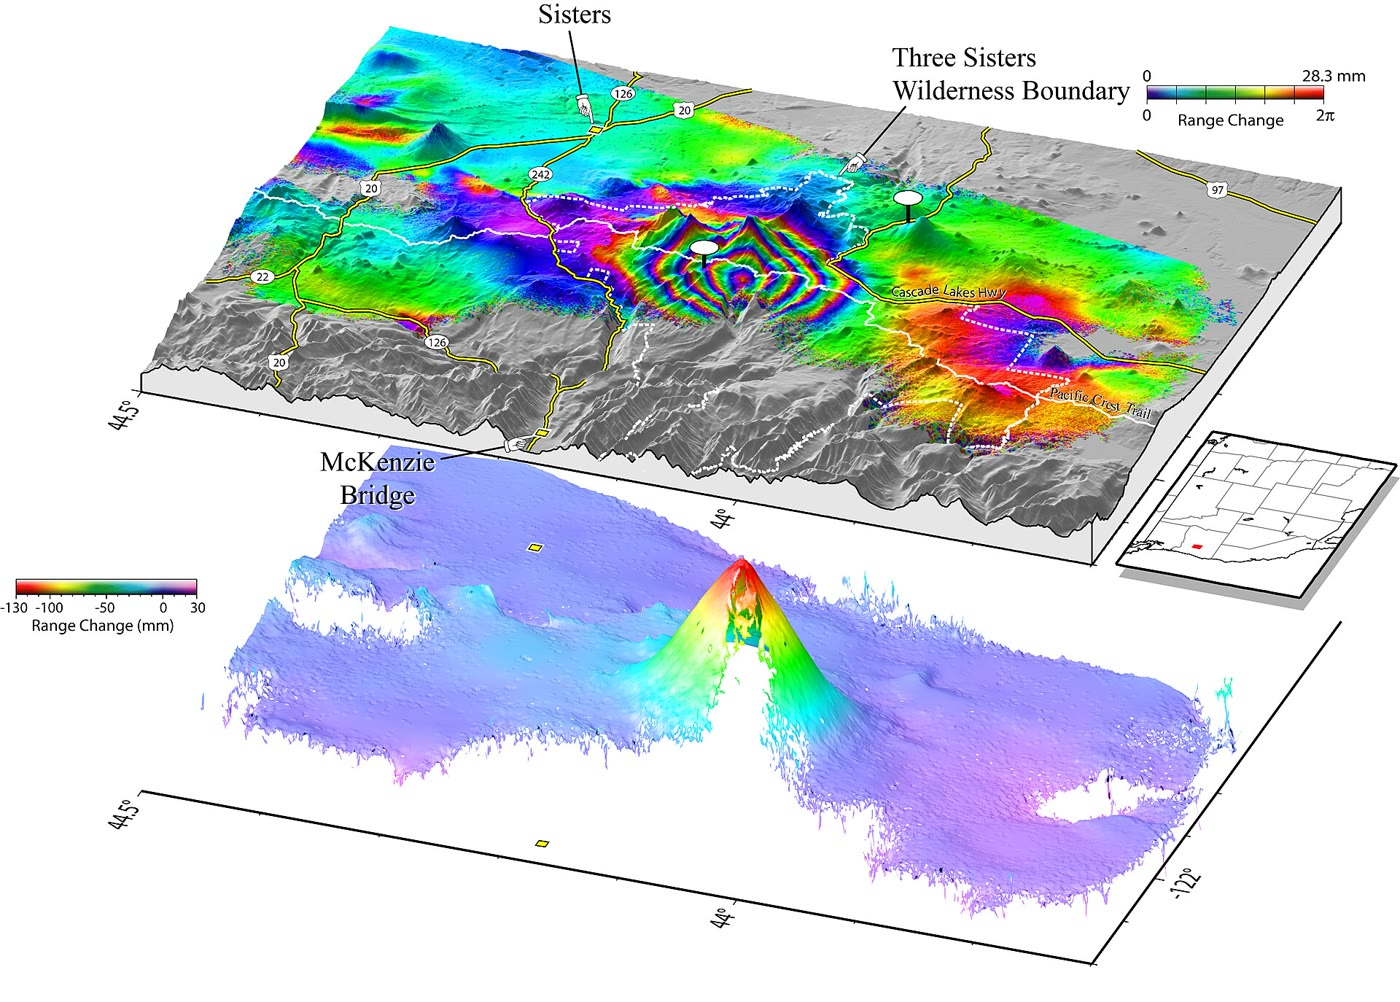
\includegraphics[width=0.86\linewidth]{images/book5/b3-three-sisters-insar.jpg}
\par\smallskip{\small Ci-dessus, l'\omterm{def:b3:remote-sensing-gis:insar}{interférogramme} du centre volcanique des Three Sisters,
Oregon, 1995--2001, drapé sur le relief~: chaque cycle de
couleurs représente \qty{28.3}{mm} de variation de distance, et l'œil de cercles
concentriques au centre marque le soulèvement. Ci-dessous, les mêmes données déroulées et figurées
en relief~: la distance au satellite diminue de jusqu'à \qty{130}{mm} au centre. U.S.
Geological Survey (Wicks et al., 2002), domaine
public.}\label{fig:b3:remote-sensing-gis:three-sisters}
\end{omfigure}
% ledger: photo:b3-three-sisters-insar, usgs:insar-fs

\begin{inthelab}[Une station au sol]
\begin{minipage}[t]{0.55\linewidth}\vspace{0pt}
Un satellite d'imagerie enregistre bien plus de données qu'il n'en peut émettre pendant qu'il survole
la zone qu'il image. Le radar d'un satellite Sentinel-1 peut imager
pendant jusqu'à une demi-heure à chaque orbite et stocke ses données à bord, jusqu'à
1410 gigabits~; il les envoie vers le sol sur deux canaux de 260 mégabits par
seconde chacun, de sorte qu'un stock plein met quelque 45 minutes à se vider. Une station au
sol les reçoit~: lorsque le satellite se lève au-dessus de l'horizon, l'antenne
parabolique s'oriente vers lui, le suit à travers le ciel et le lâche à son coucher,
tandis que les opérateurs vérifient que le flux arrive en entier. Les données partent ensuite
vers un centre de traitement, où les échos bruts deviennent des images.
\end{minipage}\hfill
\begin{minipage}[t]{0.42\linewidth}\vspace{0pt}
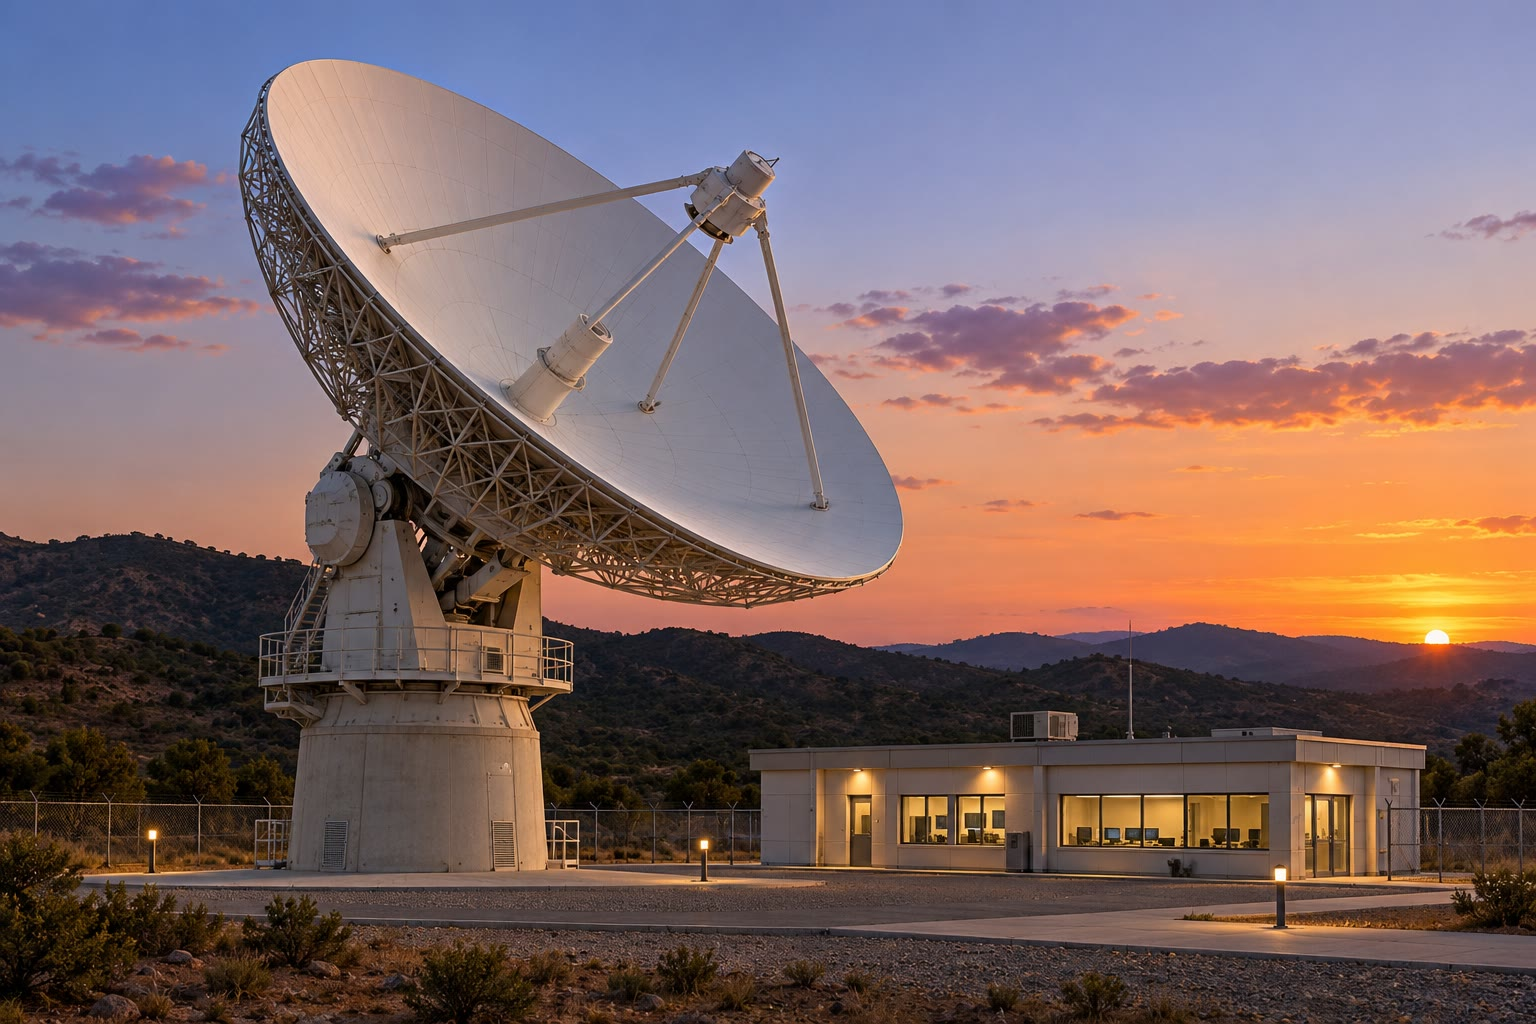
\includegraphics[width=\linewidth]{images/book5/ai/b3-ground-station.jpg}

{\scriptsize Une station au sol de satellites au crépuscule~: une grande antenne de poursuite et
son bâtiment d'exploitation (Illustration générée par IA.)}
\end{minipage}
\end{inthelab}
% ledger: esa:s1-downlink

\section{Systèmes d'information géographique}\label{sec:b3:remote-sensing-gis:gis}

Les images des satellites, le modèle numérique de terrain, la
carte géologique, les puits et les routes sont des couches d'un même
système d'information géographique, qui les stocke dans un référentiel commun de
coordonnées et calcule avec elles.

\begin{definition}[Données raster et données vectorielles]\label{def:b3:remote-sensing-gis:data-models}
Les \emph{données raster}\index{données raster} représentent une couche par une grille de
cellules, chacune portant une seule valeur~: une réflectance, une altitude, une classe.
Les \emph{données vectorielles}\index{données vectorielles (SIG)} représentent la couche par des points, des lignes
et des polygones définis par les coordonnées de leurs sommets, chacun accompagné
d'une ligne d'attributs dans une table.
\end{definition}

\begin{omfigure}
\centering
\begin{tikzpicture}[x=0.5cm, y=0.5cm, font=\scriptsize]
\begin{scope}
\draw[black!40] (0,0) rectangle (10,7);
\fill[omSea!50, draw=omDef, thick] (3,4.5) ellipse (1.8 and 1.2);
\draw[omDef, very thick] (4.8,4.5) -- (7,3.5) -- (10,2);
\fill[red!70!black] (7,5.5) circle (0.14); \fill[red!70!black] (2,1.5) circle (0.14);
\node[anchor=south] at (5,7.1) {vecteur};
\node at (3,4.5) {lac};
\node[anchor=south west] at (7.1,5.6) {puits 1};
\node[anchor=south west] at (2.1,1.6) {puits 2};
\node[anchor=north east] at (9.9,2.2) {rivière};
\end{scope}
\begin{scope}[xshift=6.5cm]
\foreach \i/\j in {1/4,2/4,3/4,4/4,2/3,3/3,2/5,3/5} {\fill[omSea!50] (\i,\j) rectangle ++(1,1);}
\foreach \i/\j in {5/4,6/3,7/3,8/2,9/2} {\fill[omDef!70] (\i,\j) rectangle ++(1,1);}
\foreach \i/\j in {7/5,2/1} {\fill[red!70!black] (\i,\j) rectangle ++(1,1);}
\draw[black!30, step=1] (0,0) grid (10,7);
\draw[black!40] (0,0) rectangle (10,7);
\node[anchor=south] at (5,7.1) {raster};
\end{scope}
\end{tikzpicture}
\par\smallskip{\small La même carte en \omterm{def:b3:remote-sensing-gis:data-models}{données vectorielles} (à gauche~: un polygone, une ligne
et deux points, exacts en position, chacun avec ses attributs) et en \omterm{def:b3:remote-sensing-gis:data-models}{données raster}
(à droite~: une valeur par cellule, le lac par les cellules dont le centre tombe à
l'intérieur du lac, la rivière et les puits par les cellules qu'ils traversent). Un raster est facile à
calculer, cellule par cellule~; une couche vectorielle conserve les formes et la topologie à
toute échelle.}\label{fig:b3:remote-sensing-gis:raster-vector}
\end{omfigure}

\begin{definition}[Géoréférencement]\label{def:b3:remote-sensing-gis:georef}
Le \emph{géoréférencement}\index{géoréférencement} est l'attribution de coordonnées cartographiques
dans une projection énoncée, à chaque pixel d'une image ou à chaque
sommet d'un dessin, le plus souvent en ajustant une transformation à des points de contrôle au sol
dont les positions sont connues dans les deux systèmes.
\end{definition}

Pour un raster orienté vers le nord dans un repère projeté, la transformation est affine~:
la cellule de la colonne $i$ et de la ligne $j$ a son coin en $E = E_0 + i\,\Delta$,
$N = N_0 - j\,\Delta$, où $\Delta$ est la taille de la cellule. Une image satellite est
d'abord rééchantillonnée dans une telle grille~; les couches dans des projections différentes sont
projetées dans une même projection avant d'être combinées.

\begin{method}[Pente, orientation et ombrage à partir d'un modèle numérique de terrain]\label{met:b3:remote-sensing-gis:slope}
Sur une grille d'altitudes $z_{i,j}$ de pas $\Delta$ ($i$ vers l'est, $j$
vers le nord), estimer le gradient par différences centrées,
\[
\frac{\partial z}{\partial x} \approx \frac{z_{i+1,j} - z_{i-1,j}}{2\Delta} ,
\qquad
\frac{\partial z}{\partial y} \approx \frac{z_{i,j+1} - z_{i,j-1}}{2\Delta} .
\]
La \emph{pente} est $S = \arctan|\nabla z|$~; l'\emph{orientation} est
l'azimut de la plus grande descente, soit la direction de $-\nabla z$, $A =
\operatorname{atan2}(-\partial z/\partial x, -\partial z/\partial y)$
mesuré dans le sens horaire à partir du nord. L'\emph{ombrage} pour une lumière
d'azimut $A_0$ à l'angle zénithal $Z$ vaut $\cos Z\cos S + \sin Z\sin S
\cos(A_0 - A)$, le cosinus de l'angle entre la lumière et la normale
au sol, ramené à zéro lorsqu'il est négatif.
\end{method}

La différence centrée est exacte pour un plan et entachée d'une erreur de
$\Delta^2 z'''/6$ sinon~; le relief ombré des monts Varden dans le
volume de première année a été calculé ainsi, éclairé depuis le nord-ouest. Les dérivées
amplifient les erreurs de la grille~: un modèle présentant des décrochements entre ses lignes
les montre sous forme de rayures sur sa carte de pente.

\begin{definition}[Algèbre de cartes]\label{def:b3:remote-sensing-gis:map-algebra}
L'\emph{algèbre de cartes}\index{algèbre de cartes} est le calcul d'une nouvelle couche raster
cellule par cellule à partir d'une ou plusieurs couches de la même grille~: par arithmétique
(le NDVI à partir de deux bandes), par comparaison (les cellules plus pentues que
\ang{15}), par opérations logiques (et, ou, non), ou à partir d'un voisinage
de la cellule (la pente).
\end{definition}

\begin{definition}[Zone tampon~; superposition]\label{def:b3:remote-sensing-gis:operations}
La \emph{zone tampon}\index{zone tampon (SIG)} d'un objet à la distance $d$ est
la région de la carte située à moins de $d$ de lui. Une
\emph{superposition}\index{superposition (SIG)} combine deux couches ou plus
d'une même zone en une seule, chaque endroit du résultat portant les attributs
de tous~; la sélection des endroits qui satisfont plusieurs conditions à la
fois, c'est l'usage le plus courant.
\end{definition}

\begin{omfigure}
\centering
\begin{tikzpicture}
\begin{groupplot}[group style={group size=2 by 2, horizontal sep=2.0cm, vertical sep=1.5cm},
  width=0.43\linewidth, axis equal image, enlargelimits=false,
  xmin=0, xmax=10, ymin=0, ymax=8,
  tick label style={font=\scriptsize}, label style={font=\small}, title style={font=\small}]
\nextgroupplot[title={(a) pente (degrés)}, ylabel={nord (km)}, colormap/viridis,
  point meta min=0, point meta max=24, colorbar right,
  colorbar style={width=0.18cm, ytick={0,5,10,15,20}, tick label style={font=\tiny}, axis equal=false}]
\addplot[matrix plot*, mesh/cols=101, point meta=explicit] table[x=x, y=y, meta=slope] {figdata/out/bachelor-3-varden_gis-grid.dat};
\addplot[white, thick] table {figdata/out/shared-region-river.dat};
\nextgroupplot[title={(b) orientation},
  colormap={aspect}{rgb255=(220,20,30) rgb255=(240,200,0) rgb255=(30,170,60) rgb255=(30,90,220) rgb255=(220,20,30)},
  point meta min=0, point meta max=360, colorbar right,
  colorbar style={width=0.18cm, ytick={0,90,180,270,360}, yticklabels={N,E,S,O,N}, tick label style={font=\tiny}, axis equal=false}]
\addplot[matrix plot*, mesh/cols=101, point meta=explicit] table[x=x, y=y, meta=aspect] {figdata/out/bachelor-3-varden_gis-grid.dat};
\addplot[black, thick] table {figdata/out/shared-region-river.dat};
\nextgroupplot[title={(c) deux couches}, xlabel={est (km)}, ylabel={nord (km)},
  colormap={lay}{rgb255=(245,245,245) rgb255=(150,150,150) rgb255=(225,195,140) rgb255=(120,70,20)},
  colormap access=piecewise constant, point meta min=-0.5, point meta max=3.5,
  legend columns=2, legend style={font=\tiny, at={(0.5,-0.3)}, anchor=north, /tikz/every even column/.append style={column sep=4pt}}]
\addplot[matrix plot*, mesh/cols=101, point meta=explicit, forget plot] table[x=x, y=y, meta=layers] {figdata/out/bachelor-3-varden_gis-grid.dat};
\addplot[omDef, thick, forget plot] table {figdata/out/shared-region-river.dat};
\addlegendimage{area legend, fill={rgb,255:red,150;green,150;blue,150}, draw=black!40}
\addlegendentry{plus pentu que \ang{15}}
\addlegendimage{area legend, fill={rgb,255:red,225;green,195;blue,140}, draw=black!40}
\addlegendentry{schiste}
\addlegendimage{area legend, fill={rgb,255:red,120;green,70;blue,20}, draw=black!40}
\addlegendentry{les deux}
\nextgroupplot[title={(d) la superposition}, xlabel={est (km)},
  colormap={cls}{rgb255=(245,245,245) rgb255=(225,195,140) rgb255=(190,150,90) rgb255=(200,20,30)},
  colormap access=piecewise constant, point meta min=-0.5, point meta max=3.5,
  legend columns=2, legend style={font=\tiny, at={(0.5,-0.3)}, anchor=north, /tikz/every even column/.append style={column sep=4pt}}]
\addplot[matrix plot*, mesh/cols=101, point meta=explicit, forget plot] table[x=x, y=y, meta=class] {figdata/out/bachelor-3-varden_gis-grid.dat};
\addplot[omDef, thick, forget plot] table {figdata/out/shared-region-river.dat};
\addplot[black, thin, dashed, unbounded coords=jump] table[x=x, y=y] {figdata/out/bachelor-3-varden_gis-buffer.dat};
\addlegendentry{zone tampon de \qty{1}{km}}
\addlegendimage{area legend, fill={rgb,255:red,225;green,195;blue,140}, draw=black!40}
\addlegendentry{schiste}
\addlegendimage{area legend, fill={rgb,255:red,190;green,150;blue,90}, draw=black!40}
\addlegendentry{schiste dans la zone tampon}
\addlegendimage{area legend, fill={rgb,255:red,200;green,20;blue,30}, draw=black!40}
\addlegendentry{sélection}
\end{groupplot}
\end{tikzpicture}
\par\smallskip{\small Une session SIG sur les monts Varden, à partir de leur modèle
numérique de terrain, sur une grille de \qty{100}{m}. (a)~La pente, jusqu'à \ang{23} sur les
flancs de la vallée~; (b)~l'orientation, la direction vers laquelle le sol fait face, les deux rives de la
rivière se faisant face~; (c)~deux couches, les cellules plus pentues que \ang{15}
et l'affleurement du schiste jurassique~; (d)~leur \omterm{def:b3:remote-sensing-gis:operations}{superposition} avec la
\omterm{def:b3:remote-sensing-gis:operations}{zone tampon} de \qty{1}{km} de la rivière (en tirets)~: les \qty{0.32}{km^2} de
schiste pentu au-dessus de la rivière, un premier crible pour les terrains susceptibles de
glisser.}\label{fig:b3:remote-sensing-gis:varden}
\end{omfigure}

La figure ci-dessus déroule toute la chaîne~: l'\omterm{def:b3:remote-sensing-gis:map-algebra}{algèbre de cartes} appliquée à la grille d'altitudes
donne la pente et l'orientation~; une comparaison transforme la pente en une couche
de cellules pentues~; la carte géologique fournit le schiste~; la \omterm{def:b3:remote-sensing-gis:operations}{zone tampon}
de la rivière donne une troisième couche~; leur intersection, une \omterm{def:b3:remote-sensing-gis:operations}{superposition} à l'aide de l'opérateur
logique \emph{et}, ne laisse que 32 cellules sur les 8181. La réponse ne vaut que par la qualité des
couches~: sur une grille plus grossière, les pentes sortent plus douces et moins de cellules passent.

\begin{definition}[Classification supervisée~; matrice de confusion]\label{def:b3:remote-sensing-gis:classification}
Une \emph{classification supervisée}\index{classification supervisée}
attribue chaque pixel d'une image à l'une des classes d'un ensemble, à partir de règles ou
de statistiques apprises sur des pixels d'apprentissage dont la classe est connue sur le terrain.
Sa \emph{matrice de confusion}\index{matrice de confusion} compte, pour un ensemble distinct
de pixels de référence, combien de pixels de chaque classe réelle ont été attribués à chaque
classe~: $n_{ij}$ pixels classés en $i$ appartiennent en réalité à $j$.
\end{definition}

La diagonale contient les pixels bien classés. Avec $N$ pixels de référence,
l'\emph{exactitude globale} vaut $\sum_i n_{ii}/N$. L'\emph{exactitude utilisateur}
d'une classe, $n_{ii}$ rapporté au total de sa ligne, est la probabilité qu'un
pixel que la carte désigne comme $i$ est réellement de classe $i$~; son \emph{exactitude producteur}, $n_{ii}$
rapporté au total de sa colonne, la probabilité qu'un $i$ réel ait été cartographié comme $i$. Le
\emph{coefficient kappa} compare l'exactitude globale $p_o$ à
l'exactitude $p_e = \sum_i (\text{ligne}_i)(\text{colonne}_i)/N^2$ qu'une attribution aléatoire
avec les mêmes totaux atteindrait~: $\kappa = (p_o - p_e)/(1 -
p_e)$.

\begin{center}
\small
\begin{tabular}{l|ccc|c}
\hline
classé \textbackslash{} référence & eau & forêt & roche nue & total \\
\hline
eau & 45 & 2 & 0 & 47 \\
forêt & 3 & 38 & 7 & 48 \\
roche nue & 0 & 5 & 30 & 35 \\
\hline
total & 48 & 45 & 37 & 130 \\
\hline
\end{tabular}
\end{center}

Dans cet exemple fictif, 113 pixels sur 130 sont bien classés, soit une exactitude
globale de \qty{86.9}{\percent}. La forêt a une exactitude utilisateur de
$38/48 = \qty{79}{\percent}$ mais une exactitude producteur de $38/45 =
\qty{84}{\percent}$~: sept pixels de roche nue, peut-être à l'ombre, ont été
classés comme forêt. Une attribution aléatoire atteindrait $p_e = 0.338$, et $\kappa =
0.80$.

\section{Exercices}

\begin{exercise}[$\star$]\label{exo:b3:remote-sensing-gis:1}
Un champ présente des réflectances de 0.06 dans la bande rouge et de 0.42 dans la
bande proche infrarouge d'un imageur~; un champ labouré voisin présente 0.21 et
0.28. Calculer le NDVI des deux et dire ce que suggère chaque valeur.
\end{exercise}

\begin{exercise}[$\star$]\label{exo:b3:remote-sensing-gis:2}
L'imageur Landsat~8 couvre une fauchée large de \qty{185}{km}, avec des pixels de \qty{30}{m}
et sa bande panchromatique, avec des pixels de \qty{15}{m}. (a)~Combien de pixels comptent une ligne
traversant la fauchée dans chaque cas~? (b)~Combien de niveaux
donnent 12 bits, et 8 bits~? (c)~Quel est le \omterm{def:b3:remote-sensing-gis:resolutions}{temps de revisite} de Landsat~8
seul, et de Landsat~8 et~9 ensemble~?
\end{exercise}

\begin{exercise}[$\star$]\label{exo:b3:remote-sensing-gis:3}
(a)~Sur un \omterm{def:b3:remote-sensing-gis:insar}{interférogramme} Sentinel-1 ($\lambda = \qty{5.55}{cm}$) d'un bassin en
subsidence, six franges séparent le bord stable du centre.
Quelle est la variation de la \omterm{def:b3:remote-sensing-gis:insar}{ligne de visée} au centre~? (b)~Que vaudrait une frange
pour un satellite plus ancien de longueur d'onde \qty{5.66}{cm}~?
\end{exercise}

\begin{exercise}[$\star$]\label{exo:b3:remote-sensing-gis:4}
Un altimètre laser est à \qty{500}{km} au-dessus du sol. (a)~Combien de temps met une
impulsion pour revenir~? (b)~Si chaque photon est repéré à \qty{800}{ps} près, quelle
est la précision d'une mesure de distance~?
\end{exercise}

\begin{exercise}[$\star\star$]\label{exo:b3:remote-sensing-gis:5}
Un pixel de la bande~10 de Landsat~8 (prendre $\lambda = \qty{10.9}{\micro\metre}$)
présente, après \omterm{def:b3:remote-sensing-gis:atm-correction}{correction atmosphérique}, une radiance spectrale de
\qty{9.0}{W.m^{-2}.sr^{-1}.\micro\metre^{-1}}. (a)~Calculer sa \omterm{def:b3:remote-sensing-gis:brightness}{température
de brillance}. (b)~La surface est un champ d'herbe d'émissivité 0.98~: quelle est
sa température cinétique~?
\end{exercise}

\begin{exercise}[$\star\star$]\label{exo:b3:remote-sensing-gis:6}
Le radar Sentinel-1 vole à \qty{693}{km} d'altitude avec une antenne de \qty{12.3}{m}
de long, à $\lambda = \qty{5.55}{cm}$. (a)~En négligeant la courbure de la
Terre, calculer la portée oblique vers un point vu sous une incidence de
\ang{35}. (b)~Quelle résolution en azimut donnerait une antenne réelle de cette longueur
à cette distance, et que donne l'ouverture synthétique~? (c)~Quelle est la
longueur de cette ouverture synthétique~?
\end{exercise}

\begin{exercise}[$\star\star$]\label{exo:b3:remote-sensing-gis:7}
Une fenêtre $3\times3$ d'un modèle numérique de terrain à cellules de \qty{30}{m}
donne, le nord en haut,
\[
\begin{matrix} 412 & 418 & 425 \\ 405 & 410 & 418 \\ 398 & 401 & 409 \end{matrix}
\qquad (\unit{m}).
\]
Par différences centrées dans la cellule centrale, calculer la pente, l'orientation
et l'ombrage du relief pour une lumière venant du nord-ouest, à \ang{45} au-dessus de
l'horizon.
\end{exercise}

\begin{exercise}[$\star\star$]\label{exo:b3:remote-sensing-gis:8}
Une carte d'occupation des sols est vérifiée par rapport à 160 pixels de référence (lignes~: la carte~;
colonnes~: la réalité~; classes eau, forêt, cultures, zone urbaine)~:
\[
\begin{pmatrix} 48 & 3 & 1 & 0 \\ 4 & 37 & 6 & 1 \\ 2 & 5 & 29 & 2 \\ 0 & 1 & 2 & 19 \end{pmatrix} .
\]
Calculer l'exactitude globale, les exactitudes utilisateur et producteur de chaque
classe, et le coefficient kappa. Quelle classe est la plus souvent manquée~?
\end{exercise}

\begin{exercise}[$\star\star$]\label{exo:b3:remote-sensing-gis:9}
Un pixel thermique de \qty{100}{m} contient une coulée de lave fraîche à \qty{1443}{K},
couvrant \qty{4}{\percent} de sa surface~; le reste est du sol à \qty{290}{K}~; considérer
les deux comme des corps noirs. (a)~Calculer la \omterm{def:b3:remote-sensing-gis:brightness}{température de brillance} du pixel
à \qty{10.9}{\micro\metre} et la comparer à la température moyenne.
(b)~Calculer le rapport des radiances de corps noir de la lave et du
sol à \qty{2.2}{\micro\metre}, ainsi que la \omterm{def:b3:remote-sensing-gis:brightness}{température de brillance} du
pixel dans cette bande. Quelle bande détecte mieux la lave~?
\end{exercise}

\begin{exercise}[$\star\star\star$]\label{exo:b3:remote-sensing-gis:10}
Deux \omterm{def:b3:remote-sensing-gis:insar}{interférogrammes} de la même déformation sont produits à partir de deux passages, l'un
avec le satellite à l'est du sol et l'autre avec le satellite à l'ouest,
tous deux sous une incidence de \ang{35}. En un point, la
\omterm{def:b3:remote-sensing-gis:insar}{ligne de visée} raccourcit de \qty{64}{mm} sur le premier et de \qty{38}{mm} sur
le second. En supposant nul le mouvement nord--sud, calculer les déplacements vertical et
vers l'est. Pourquoi un seul passage ne suffit-il pas~?
\end{exercise}

\begin{exercise}[$\star\star\star$]\label{exo:b3:remote-sensing-gis:11}
Le \omterm{def:b3:remote-sensing-gis:insar}{déroulement de phase} échoue lorsque la phase saute de plus de $\pi$ entre
pixels voisins. (a)~Montrer que la \omterm{def:b3:remote-sensing-gis:insar}{ligne de visée} doit varier de moins de
$\lambda/4$ d'un pixel au suivant, soit \qty{13.9}{mm} pour
Sentinel-1. (b)~Pour une source de Mogi à $z_0 = \qty{4}{km}$ avec $\Delta V =
\qty{e7}{m^3}$ et $\nu = 0.25$, vue à la verticale, montrer que le gradient maximal
de $u_z$ se situe en $r = z_0/2$, et en calculer la valeur. (c)~Quelle est la
plus grande taille de pixel qui permet de résoudre les franges~?
\end{exercise}

\begin{exercise}[$\star\star\star$]\label{exo:b3:remote-sensing-gis:12}
(a)~Montrer que le NDVI est compris entre $-1$ et $+1$ pour des réflectances
positives ou nulles, et qu'il reste inchangé lorsque les deux réflectances sont
multipliées par un même facteur. (b)~L'herbe présente des réflectances de 0.051 (rouge)
et 0.502 (proche infrarouge). Une image non corrigée ajoute une radiance de trajet
équivalente à 0.03 dans le rouge et 0.01 dans le proche infrarouge. Calculer le
NDVI avec et sans cette contribution. (c)~Quelles conséquences cela a-t-il pour une carte du NDVI
établie à partir d'images non corrigées par temps brumeux~?
\end{exercise}

\section{Problème~: un flanc en gonflement au mont Halvren}

\begin{problem}[{Problème du week-end --- végétation, chaleur et radar
interférogramme sur un volcan fictif}]
\label{pb:b3:remote-sensing-gis:1}
Le mont Halvren, volcan fictif, a produit des coulées de lave en 1890, en 1960
et en 2005 sur ses flancs boisés. Un champ de fumerolles dégage de la vapeur à son sommet.
Des données satellitaires d'une année récente sont fournies ci-dessous.

\medskip\noindent\textbf{Partie I --- Végétation sur les coulées de lave.} Réflectances corrigées
dans les bandes rouge et proche infrarouge~:
\begin{center}
\small
\begin{tabular}{lcccc}
\hline
surface & forêt & coulée de 1890 & coulée de 1960 & coulée de 2005 \\
\hline
rouge & 0.04 & 0.07 & 0.11 & 0.12 \\
proche infrarouge & 0.38 & 0.30 & 0.21 & 0.14 \\
\hline
\end{tabular}
\end{center}
\begin{enumerate}
\item Calculer le NDVI des quatre surfaces.
\item Classer les coulées selon la \omterm{def:b3:deformation-mechanisms:recrystallisation}{restauration} de leur végétation. Ce classement est-il
  celui de leurs âges~?
\item Pourquoi le NDVI de la coulée de 2005 n'est-il pas nul, alors que presque
  rien ne pousse dessus~?
\item Pourquoi le NDVI est-il plus fiable que la seule réflectance dans le proche infrarouge
  sur les flancs raides et inégalement éclairés d'un volcan~?
\end{enumerate}

\medskip\noindent\textbf{Partie II --- Le champ de fumerolles.} Dans la bande
thermique (prendre $\lambda = \qty{10.9}{\micro\metre}$), la radiance corrigée de
un pixel de \qty{100}{m} du plateau sommital, loin des fumerolles, est
\qty{8.40}{W.m^{-2}.sr^{-1}.\micro\metre^{-1}}, et celle du pixel au-dessus
du champ de fumerolles \qty{9.95}{W.m^{-2}.sr^{-1}.\micro\metre^{-1}}.
\begin{enumerate}[resume]
\item Calculer les \omterm{def:b3:remote-sensing-gis:brightness}{températures de brillance} des deux pixels.
\item La roche du plateau a une émissivité de 0.97. Quelle est sa température
  cinétique~?
\item Les évents des fumerolles et le sol chaud qui les entoure sont à
  \qty{370}{K}. En les traitant, ainsi que le reste du pixel, comme des corps noirs,
  le reste étant à la radiance du plateau, quelle fraction du pixel occupent-ils
  et quelle aire cela représente~?
\item Pourquoi la température moyenne du pixel, pondérée par les surfaces, est-elle inférieure
  à sa \omterm{def:b3:remote-sensing-gis:brightness}{température de brillance}~?
\end{enumerate}

\medskip\noindent\textbf{Partie III --- L'interférogramme.} Deux
images Sentinel-1 ($\lambda = \qty{5.55}{cm}$, incidence \ang{35}, satellite à
l'est) prises à 48 jours d'intervalle montrent un motif en œil-de-bœuf sur le flanc est. Depuis une
zone stable jusqu'au centre du motif, on compte cinq franges entières et
quatre dixièmes d'une sixième, toutes dans le sens du mouvement vers le
satellite.
\begin{enumerate}[resume]
\item Pourquoi deux images doivent-elles être prises depuis une position presque identique, et combien
  de cycles orbitaux d'un même satellite les séparent~?
\item Calculer la variation de la \omterm{def:b3:remote-sensing-gis:insar}{ligne de visée} au centre.
\item Au centre, le sol ne se déplace que verticalement. Calculer le soulèvement
  en ce point.
\item Expliquer pourquoi le motif n'est pas circulaire, et de quel côté, est ou
  ouest, les franges sont les plus serrées.
\item Le long de la ligne nord--sud passant par le centre, la variation de la
  \omterm{def:b3:remote-sensing-gis:insar}{ligne de visée} tombe à la moitié de sa valeur centrale à \qty{3.4}{km} du
  centre. Pourquoi utiliser cette ligne, et quelle profondeur donne-t-elle pour une
  source de Mogi~?
\item Combien de franges séparent le centre de ce point situé à mi-hauteur~?
\item La vapeur d'eau de l'air peut retarder différemment les ondes radar aux
  deux dates et former ses propres franges. Comment un second \omterm{def:b3:remote-sensing-gis:insar}{interférogramme},
  construit à partir d'un autre couple de dates, aiderait-il à les distinguer~?
\end{enumerate}

\medskip\noindent\textbf{Partie IV --- Le volume.} Prendre $\nu = 0.25$.
\begin{enumerate}[resume]
\item À partir de $u_z(0) = (1 - \nu)\Delta V/(\pi z_0^2)$, calculer la variation de volume
  de la source.
\item L'exprimer comme un taux moyen par jour et par an sur les 48 jours.
\item Calculer le plus grand déplacement horizontal et l'endroit où il se produit.
\item Si le réservoir était une sphère de rayon $z_0/3$, quel serait son volume
  et quelle fraction de celui-ci représente la variation~?
\item La taille finie d'une sphère de rayon $z_0/3$ modifie le soulèvement d'environ
  \qty{3}{\percent}. Modifie-t-elle sensiblement la réponse à la question~16
  compte tenu de la précision du comptage des franges~?
\item Quelle autre observation, issue des parties I et II ou du terrain,
  appuierait l'interprétation d'un réservoir en cours de remplissage~?
\item Donner la variation de volume du réservoir sous le mont Halvren, en
  millions de mètres cubes, à deux chiffres significatifs.
\end{enumerate}
\end{problem}
% ledger: nasa:ndvi, esa:s1-sar, esa:s1-orbit, esa:s1-iw, dmodels:mogi, dmodels:mogi-radial, const:h, const:c, const:kB
